%--- Begin generated contents ---
\chapter{The discontinuous Galerkin spectral element method}
CMT-nek is an implementation of the
\textbf{discontinuous Galerkin spectral element method (DGSEM)} written for
systems of conservation laws. General descriptions and theory of DG methods is
found in a few textbooks. I recommend \cite{hw08,CHQZ3}, where much of the notation
in this document is taken.
It solves for 5 conserved variables $\bU(\mathbf{x},t) \in \mathbb{R}^5$, 
$\mathbf{x} =\left(x_1,x_2,x_3\right)^{\Txp} \in \Omega \subset \mathbb{R}^3$, $t\in\mathbb{R}^+$,
satisfying the conservation law
\begin{equation}
\pp{\bU}{t} + \divnce \bH=\mathbf{R},
\label{claw}
\end{equation}
where each of the 5 equations has its own flux vector
$\bH(\bU) : \bU \rightarrow \mathbb{R}^3$.

\section{The discontinuous Galerkin spectral element method (DGSEM)\label{sec:dgsem}}
CMT-nek solves Equation~\ref{claw} by partitioning the
domain $\Omega \subset \mathbb{R}^d$, $d={1,2,3}$  into nelt non-overlapping elements (Figure~\ref{elements}),
the $e$\textsuperscript{th} of which is $\Omega_e$,
and marching the left-hand-side of Equation~\ref{claw} forward in time on
each element. The right-hand-side of Equation~\ref{claw} is discretized on
each element in a very peculiar way called \textbf{the two-point form of DGSEM}
that is only briefly summarized here.
The two-point form of DGSEM brings discontinuous Galerkin methods and finite
difference methods together in a very peculiar way, and the reader is strongly encouraged to study the bibliography carefully.

\subsection{Weighted residuals\label{sec:wrt}}
Galerkin methods force an inner product of Equation~\ref{claw} with a test function to vanish
for every value of the test function in some basis spanning a finite-dimensional
space of test functions $\chi$.
Integrating this inner product by parts on a given element$\Omega_e$ gives us the \textbf{weak form} of the discontinuous Galerkin weighted residual
statement for the governing equation~\ref{claw}:
\begin{equation}
\int_{\Omega_e} v(\bx) \pp{\bU(\bx)}{t}dV = 
\int_{\Omega_e} \left(\nabla v\right) \cdot \bH\, dV  
-\int_{\dO_e} v(\bx) \bH^{\ast}(\bU^-,\bU^+) \cdot \bhn dA +
\int_{\Omega_e} \mathbf{R}(\bx) v(\bx) dV,
\label{dghweak}
\end{equation}
where the surface integral term $\bH\cdot\bhn$ in the surface integral has been replaced by
the \textbf{numerical flux} $\bH^{\ast}(\bU^-,\bU^+)\cdot \bhn$ that, since $\chi$
is a broken space defined on each element, resolves the discontinuities between
the representation of $\bU$ on the faces of $\Omega_e$ and the corresponding $\bU$
in the neighbors sharing faces $f \in \dO_e$. That is,
\begin{align}
   U^-(\bx) \equiv & U(\bx) \mbox{ taken from the \textbf{interior}, or trace, of }\Omega_e \label{uminus}\\
   U^+(\bx) \equiv & U(\bx) \mbox{ taken from the \textbf{element adjacent to} }\Omega_e\mbox{ sharing }\dO_e. \label{uplus}
\end{align}
The numerical flux functon $\bH^{\ast}$ is critically important to the stability
and convergence properties of DGSEM, and will be presented in more detail in
\S\ref{}.

\begin{figure}
\centering
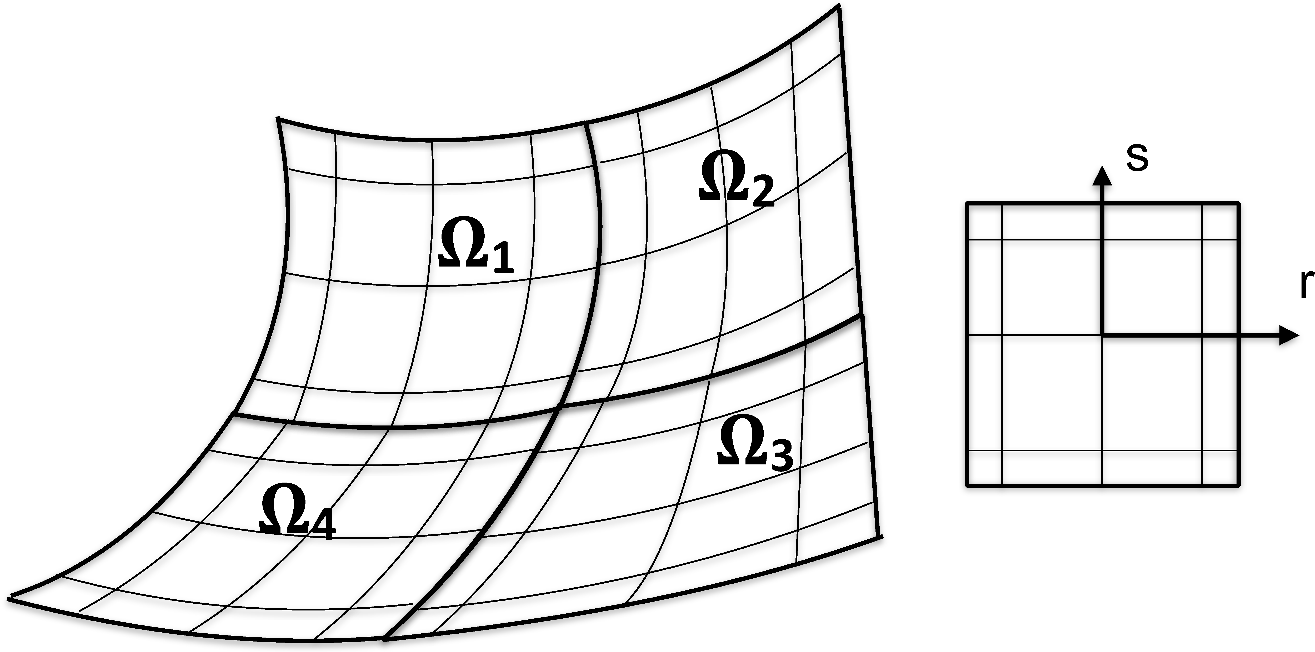
\includegraphics[width=8.0cm]{elements}
\caption{A schematic representation of spectral elements and the reference element in two dimensions.}
\label{elements}
\end{figure}

Figure~\ref{elements} also illustrates how a point $\bx\in\Omega_e$ is isoparametrically mapped to
$\mathbf{r}\equiv\left(r,s,t\right)^{\Txp}=\left(r_1,r_2,r_3\right)^{\Txp}$ in the reference element
$\Oh=[-1,1]^3$,
This transformation has, $\forall \mathbf{x}\in\Omega_e$,
Jacobian $J(\mathbf{x})\equiv|\partial \mathbf{x}/\partial \mathbf{r}|$ and
metrics $\partial r_i/\partial x_j$.

We integrate the right-hand-side (RHS) of Equation~\ref{dghweak} by parts a second time to get
the \textbf{``strong'' form} of the weighted residual statement,
\begin{equation}
\int_{\Omega_e} v(\bx) \pp{\bU(\bx)}{t}dV = 
\int_{\Omega_e} v \nabla \cdot \bH\, dV  
-\int_{\dO_e} v(\bx) \left(\bH-\bH^{\ast}\right) \cdot \bhn dA +
\int_{\Omega_e} \mathbf{R}(\bx) v(\bx) dV.
\label{dghstrong}
\end{equation}
The distinction between weak and strong forms is ultimately unimportant in DGSEM,
but strong form (Equation~\ref{dghstrong}) is clearer and more convenient.

\subsection{Quadrature and approximation}
All integrals in Equation~\ref{dghstrong} are now approximated by
\textbf{Gaussian quadrature}, as described in \S whatever of \cite{dfm02}.
We evaluate the solution $\bU$ and various functions of it (like fluxes $\bH$ and
source terms $\mathbf{R}$) on a grid of $N^3$ \textbf{Gaussian quadrature nodes}
within each element. This means:
\begin{enumerate}
\item The approximation space $\chi$ becomes $[\mathbb{P}^{N-1}]^3$, a Cartesian product of the space of all
polynomials of degree $N-1$.
\item The basis functions are a \textbf{nested tensor product} of the \textbf{interpolating Lagrange
polynomials} evaluated on $N^2$ lines of $N$ Gaussian quadrature nodes. This is
described in more detail in \S of \cite{dfm02}.
\item The discrete unknowns are the \textbf{nodal values} $\bU(x_i,y_j,z_k)$ at each of the $N^3$ Gaussian nodes in each element.
\end{enumerate}
Finally, within the family of Gaussian quadrature we specifically choose the
\textbf{Gauss-Legendre-Lobatto (GLL)} nodes. Formulas for $\omega$ and $\mathbf{r}$ may be found in Appendix of \cite{dfm02}.

Nodal values at grid points within a given element are arranged into
vectors lexicographically:
\begin{equation}
\mathbf{u}\equiv\left[\begin{array}{c} U(x_1,y_1,z_1) \\  U(x_2,y_1,z_1) \\ \vdots \\ U(x_N,y_N,z_N) \end{array}\right],
\mathbf{v}\equiv\left[\begin{array}{c} v(x_1,y_1,z_1) \\ v(x_2,y_1,z_1) \\  \vdots \\ v(x_N,y_N,z_N) \end{array}\right],
\mathbf{h}_1\equiv\left[\begin{array}{c} H_x(U(x_1,y_1,z_1))\\ H_x(U(x_2,y_1,z_1))\\   \vdots \\ H_x(U(x_N,y_N,z_N)) \end{array}\right],
\label{gridvects}
\end{equation}
with $u_l=U(x_i,y_j,z_k)$ when $l=i+N(j\!-\!1)+N^2(k\!-\!1)$.

These vectors may be catenated one element after the other into a vector $\buu_L$ of $N^3 K$ nodal
values for
the quadrature nodes in the entire mesh.

To assist notation for scalar multiplication, we introduce the diagonal matrix formed
from an arbitrary nodal vector $\mathbf{f}$
\begin{equation}
\mbox{diag}(\mathbf{f})\equiv \left[\begin{array}{cccc} f(x_1,y_1,z_1) & & & 0 \\
                                                        & \diagdown & & \\ 
                                                        & & f(x_i,y_j,z_k)  & \\
                                                        & & \diagdown & \\
                                                        & & & \\
                                                        0 & & & f(x_N,y_N,z_N)\end{array}\right].
\label{diagalot}
\end{equation}

Consider the left-hand-side of Equation~\ref{dghstrong}. Approximating everything with
the nodal representation on $N^3$ GLL points described above,
means our discrete equation becomes, at the top level,
\begin{equation}
\int_{\Omega_e} v(\bx) \pp{\bU(\bx)}{t}dV \approx \bv^{\Txp}\mathbf{B}\pp{\bu}{t} =
\mbox{RHS},
\label{firstdiscrete}
\end{equation}
where RHS is the right-hand-side of Equation~\ref{dghstrong}
evaluated at each GLL node. Bold-faced quantities are nodal vectors (Equation~\ref{gridvects}) including
the mass matrix $\mathbf{B}$,
\begin{equation}
\mathbf{B}\equiv \left[\begin{array}{ccc} \diagdown & & 0 \\ &  \omega_i\omega_j\omega_k J(\mathbf{x}(r_i,s_j,t_k)) &  \\  0 & & \diagdown \end{array}\right],
\label{masslex}
\end{equation}
where $\omega_i$ is the GLL quadrature weight associated with the $i$\nth quadrature
node,
and $J_e(\mathbf{x})$ is the Jacobian $J$ of the mesh transformation described
above at the GLL points within $\Omega_e$.

The Galerkin statement is enforced for all possible test functions in $\chi$ by
equating coefficients of the test function $\mathbf{v}$ on both sides of Equation~\ref{firstdiscrete}.
%\textbf{It suffices for me to state that
%any operation in the volume integral in Equation~\ref{dghstrong} using the transpose
%of a matrix or a Kronecker product labeled as a transpose is really being applied to the test functions.}
Further multiplication of Equation~\ref{firstdiscrete} by $\mathbf{B}^{-1}$ produces the semidiscrete method of lines
\begin{equation}
\pp{\bu}{t} =\mathbf{B}^{-1}\mbox{RHS}=I_{\mbox{vol}}-I_{\mbox{sfc}},
\label{dgsemifinal}
\end{equation}
which may be integrated in time to solve for the nodal values $\bu$ of the conserved variables.
Right-hand-side terms in Equation~\ref{dgsemifinal} are essentially the effects
contributions of individual GLL nodes to integrals (hence the ``I''
abbreviation). We describe those in the following section.

\section{Split forms of evaluating summation-by-parts operators\label{splitform}}
% MAKE SURE
%\bh and \bH are not confused
%\bh_m is used where appropriate for a nodal vector of a single unknown's flux
% H_m
We're solving a differential equation. We need to take derivatives of things
like $U$ and $\mathbf{H}$ approximated by polynomials on each element.
Finite differences are appropriate for computing derivatives of interpolating polynomials.
Algorithms are commonplace for finite differences on each of $N$ points expressed as
products between a $N\times N$ differentiation matrix $\mathcal{D}$ and a
vector of $N$ nodal values in one spatial dimension,
\begin{equation}
\mathcal{D}\bv \approx\left[\left.\dd{v}{r}\right|_{r_1},\, \cdots,\,\left.\dd{v}{r}\right|_{r_N} \right]^{\Txp}.
\label{diffmat1D}
\end{equation}
$\mathcal{D}$ is computed in Nek5000 using formulas derived in \cite[\S]{dfm02}.

Derivatives of $U$ for all $N^3$ GLL nodes in $\Omega_e$ in each of the three coordinate directions on
$\Oh$ are evaluated via the triple Kronecker product (see \cite[\S]{dfm02}) of $\mathcal{D}$ with
$\mathbf{I} \in\mathbb{R}^{N\times N}$:
\begin{equation}
\mathbf{D}_r=\mathbf{D}_{r_1}=\mathbf{I}  \otimes \mathbf{I} \otimes \mathcal{D}, \quad
\mathbf{D}_s=\mathbf{D}_{r_2}=\mathbf{I}  \otimes \mathcal{D}\otimes \mathbf{I} , \quad
\mathbf{D}_t=\mathbf{D}_{r_3}=\mathcal{D} \otimes \mathbf{I} \otimes \mathbf{I}.
\label{diffkron}
\end{equation}

On the GLL nodes, $\mathcal{D}$ has the \textbf{summation-by-parts property}:
\begin{equation}
\left(\mathbf{B}\mathcal{D}\right)^{Txp}+\mathbf{B}\mathcal{D}=\mbox{diag}\left(\left[-1,0,\dots,0,1\right]\right),
\label{SBP}
\end{equation}
which means that integration by parts in inner products like Equations~\ref{dghweak} and~\ref{dghstrong}
is done \emph{exactly} at the discrete level \emph{even if} 
the underlying quadrature is not itself exact.
Na{\"i}vely, we would write $I_{\mbox{vol}}$ in Equation~\ref{dgsemifinal} by
approximating the volume integral\footnote{The Einstein summation convention
applies to multiplication of derivatives in the direction $i$ on the GLL grid with flux in the
physical direction $j$.}
\begin{equation}
\sum_{e=1}^{nelt}\int_{\Omega_e} v \nabla \cdot \bH\, dV \approx
\bv^{\Txp}\mathbf{B}\mathbf{D}_i\left[\mbox{diag}\left(\frac{\partial r_i}{\partial x_j}\right)\bh_j\right],
\label{badvolint}
\end{equation}
where $\bh_j$ is the flux in the $x_j$ direction at the GLL nodes on all elements. We would then equate coefficients of $\bv$ and left multiply by
$\mathbf{B}^{-1}$ to get $I_{\mbox{vol}}$. However, it turns out\cite{CarpenterESSC} Equation~\ref{badvolint}
is itself further approximated by \textbf{a subcell flux difference}. Considering
a single GLL grid line on an undeformed element (such that $r=x_1$ for brevity, Fisher\cite{FisherJCP252}
proved\footnote{Cartesian indices in parentheses like ``$(i)$'' refer to the
$i^{\mbox{th}}$ element of an array and are \emph{not} subject to summation
convention.}
\begin{equation}
\left(\mathbf{D}_r\mathbf{h}_r\right)_{(ijk)}\approx
\frac{F_{(i+1,jk)}-F_{(ijk)}}{\omega_i}
\label{travis}
\end{equation}
to within the truncation error of the Lagrange polynomials on GLL nodes
with nodal values of fluxes $\bh$. Fisher introduced a \textbf{auxiliary flux function} $F$
that provided a way of enforcing bounds on fluxes \emph{even in the face of
quadrature errors in evaluating them.} The importance of this for stabilization
will be discussed in \S.

Finally, Fisher derived a \textbf{two-point split form} for Equation~\ref{travis}
that allowed (further) approximation of $F$ with \emph{yet another} flux function $F^{\#}$
\begin{equation}
\frac{F_{(i+1,jk)}-F_{(ijk)}}{\omega_i}\approx 2
\sum_{l=1}^N\mathcal{D}_{il}F^{\#}\left(\bu_{(ijk)},\bu_{(ljk)}\right),
\label{finally2pt}
\end{equation}
where $F^{\#}\left(\bU_a,\bU_b\right)$ is a flux function of two arguments instead of one!
At the very least, it must be consistent with the physical flux function.
%given conserved variable (numbered $m\in[1,5]$ below):
\begin{equation}
%F_m^{\#}\left(\bU,\bU\right)=H_m(\bU)
\bF^{\#}\left(\bU,\bU\right)=\bH(\bU)
\label{consistency}
\end{equation}
and symmetric in its two arguments.

So, to summarize, Equation~\ref{finally2pt} is, for system-dependent choices of
$\mathbf{F}^{\#}$ to be shown in \S, a \emph{stabilizing} way of approximately
evaluating the volume integral in Equation~\ref{dghstrong} for schemes based on
summation-by-parts (SBP) operators. Finite differences on GLL nodes in DGSEM are
SBP operators. While Equation~\ref{finally2pt} disrupts the matrix-vector
product $\mathbf{Du}$, it retains $N^4$ scaling in higher dimensions and promises
some unique stability properties on top of conservation and high-order accuracy\cite{walchidk}.
As a notational shorthand, we abbreviate Equation~\ref{finally2pt} as
\begin{equation}
\mathbb{D}(F^{\#})\equiv 2
\sum_{l=1}^N\mathcal{D}_{il}F^{\#}\left(\bu_{(ijk)},\bu_{(ljk)}\right),
\label{theotherd}
\end{equation}
where $F^{\#}\left(\bU_a,\bU_b\right)$ is a flux function of two arguments instead of one!
At the very least, it must be consistent with the physical flux function for a

Gassner, Winters and Kopriva\cite{splitformnodaldg} (and the works cited therein)
derive and explore several properties and features of these
``\textbf{two-point split forms}'' for the Euler equations. They transform them
to deformed spectral elements as follows.
Let indices \emph{i,j,k,l} denote individual GLL nodes within $\buu$ in three-dimensional storage or matrix elements.
First, fluxes must be transformed in a freestream-preserving way into the
\textbf{contravariant frame} aligned along the GLL grid within a given element.
Again, we subscript $\bH=\left(\bH_1,\bH_2,\bH_3\right)$ by the physical-space
direction $j\in[1,3]$. Again, we distinguish Cartesian tensor indices from GLL
nodes and matrix elements by writing, for example, the $x_2$-direction flux at
the $i^{\mbox{th}}$ GLL node as $H_2\left(\bU_{(i)}\right)$ and \emph{demanding
that summation convention apply} to the index on $H$ but \emph{NOT} to the
index on $\bU$!!!
Then, for a given conserved variable, the integrand in the volume integral in Equation~\ref{dghstrong} becomes
% DONT CRY. PiCK YOURSELF UP OFF HTE FLOOR. NOW
% ANSWER ONE QUESTION
% IS rx MULTIPLIED BY J IN THE 2-POINT CODE OR NOT?
\begin{equation}
\left[\mathbf{D}_r\mathbf{h}\right]_{(ijk)}\approx
\left[\mathbb{D}_r\left(F^{\#}\right)\right]_{(ijk)}\equiv
2\sum_{l=1}^N\mathcal{D}_{(il)}
\left\{\left\{J\mbox{diag}\left(\frac{\partial r_1}{\partial x_k}\right)\right\}\right\}_{((i,l)jk)}F^{\#}_k\left(\bU_{(ijk)},\bU_{(ljk)}\right),
\label{splitr}
\end{equation}
\begin{equation}
\left[\mathbf{D}_s\mathbf{h}\right]_{(ijk)}\approx
\left[\mathbb{D}_s\left(F^{\#}\right)\right]_{(ijk)}\equiv
2\sum_{l=1}^N\mathcal{D}_{(jl)}
\left\{\left\{J\mbox{diag}\left(\frac{\partial r_2}{\partial x_k}\right)\right\}\right\}_{(i(j,l)k)}F^{\#}_k\left(\bU_{(ijk)},\bU_{(ilk)}\right),
\label{splits}
\end{equation}
\begin{equation}
\left[\mathbf{D}_t\mathbf{h}\right]_{(ijk)}\approx
\left[\mathbb{D}_t\left(F^{\#}\right)\right]_{(ijk)}\equiv
2\sum_{l=1}^N\mathcal{D}_{(kl)}
\left\{\left\{J\mbox{diag}\left(\frac{\partial r_3}{\partial x_k}\right)\right\}\right\}_{(ij(k,l))}F^{\#}_k\left(\bU_{(ijk)},\bU_{(ijl)}\right),
\label{splitt}
\end{equation}
% DONT CRY. PiCK YOURSELF UP OFF HTE FLOOR. NOW
% ANSWER ONE QUESTION
% IS rx MULTIPLIED BY J IN THE 2-POINT CODE OR NOT?
where we have introduced notation for an \textbf{average} between two grid points
along a line of fixed $r$ in the grid on the reference element,
\begin{equation}
\left\{\left\{U\right\}\right\}_{((i,l)jk)}\equiv\frac{1}{2}\left(U_{(ijk)}+U_{(ljk)}\right),
\label{avgr}
\end{equation}
\begin{equation}
\left\{\left\{U\right\}\right\}_{(i(j,l)k)}\equiv\frac{1}{2}\left(U_{(ijk)}+U_{(ilk)}\right),
\label{avgs}
\end{equation}
\begin{equation}
\left\{\left\{U\right\}\right\}_{(ij(k,l))}\equiv\frac{1}{2}\left(U_{(ijk)}+U_{(ijl)}\right).
\label{avgt}
\end{equation}
These averages will be needed to define various flux functions of interest too. Equations~\ref{splitr} through~\ref{splitt} are applied component-wise to each of the conserved variables in
$\mathbf{H}$ (with correponding components in $\mathbf{F}$).

So, we have an elaborate way of writing the discrete approximation to the
volume integral on the right-hand-side of Equation~\ref{dgsemifinal}:
\begin{equation}
I_{\mbox{vol}}\equiv \mbox{diag}\left(\frac{1}{J}\right)\sum_{j=1}^3\mathbb{D}_j\bh
\label{shortvol}
\end{equation}
where $\mathbb{D}_j$ is defined by Equations~\ref{splitr} through~\ref{splitt}.

\subsection{A short note on strong form}
The extra discontinuous surface flux in Equation~\ref{dghstrong} is evaluated
on the fly by modifying the differentiation matrix $\mathcal{D}$. In the
code,
\begin{equation}
dstrong=\mathcal{D}-2\mbox{diag}\left(\left[-1/\omega_1,0,\dots,0,1/\omega_N\right]\right)\mathbb{D}
\label{dstrong}
\end{equation}
is enough to include the surface integral from integrating by parts twice. dstrong
is evaluated in chainrule\_metrics subroutine of intpdiff.
%LINK THAT

%The general flux function for all 5 governing equations is now noted 

\section{Surface integral terms}%\label{sfcmath}}\index{Surface\_math@{Surface\_math}}
%INDEX YOUR SHIT!!!
\begin{equation}
I_{\mbox{sfc}}=-\left(\sum_{f=1}^6
\mathbf{E}^{(f)\Txp}\mathbf{B}^{(f)}\left[\mbox{diag}\left(\bhn^{(f)}_j\right)\left(\bh_j-\bh^{\ast(f)}_j\right)\right]\right).
\label{isfc} % was dgweak
\end{equation}
where the ``face'' mass matrix $\mathbf{B}^{(f)}$ is
\begin{equation}
\mathbf{B}^{(f)}\equiv \left[\begin{array}{ccc} \diagdown & & 0 \\ &  \omega_i\omega_j J^{(f)}(\mathbf{x}(r_i,s_j)) &  \\  0 & & \diagdown \end{array}\right]\in\mathbb{R}^{N^2 \times N^2},
\label{massA}
\end{equation}
and we note that the vectors of nodal values $\bhn^{(f)}_j$ and $\bh^{(f)}_j$ in
\ref{isfc} have only $N^2$ elements since they correspond to GLL nodes on face $f$.
Crucially, we have also introduced the \emph{restriction operator} $\mathbf{E}^{(f)}\in\mathbb{R}^{N^2\times N^3}$ for the $f^{\mbox{th}}$ face in \ref{isfc}.
The restriction operator is defined as an indicator that is zero for all GLL nodes except those on the
element faces $\dO_e$, an operation easily expressed as Kronecker products (for example, in the
$r_1-$direction for $f=1$ at $r=r_1=-1$)
\begin{equation}
\bE^{(1)}=\bI\otimes \bI\otimes \mathcal{E}_1
\label{bigE1}
\end{equation}
of the $\bI\in\mathbb{R}^{N\times N}$ identity matrix with unit vectors $\mathcal{E}\in\mathbb{R}^N$
(in \ref{bigE1}, $\mathcal{E}_1\equiv\left(1,0,\dots, 0\right)^{\Txp}$).
Similar indicators may be built up in the $r_2$- and $r_3$-directions by following the ordering of
Kronecker products in \ref{diffkron}.
%Substituting \ref{isfc} into~\ref{sfcintcube} and applying the matrix identity $(\bA\bB)^{\Txp}=\bB^{\Txp}\bA^{\Txp}$ discretely represents the surface integral of the numerical flux on $\Oh$:
Applying the matrix identity $(\bA\bB)^{\Txp}=\bB^{\Txp}\bA^{\Txp}$ to Equation~\ref{isfc} discretely represents the surface integral of the numerical flux on $\Oh$:
\begin{equation}
\sum_{f=1}^6\iint\displaylimits_{-1}^1 v(\br) H^{\ast(f)}_j\hat{n}^{(f)}_j J^{(f)}\, dr \, ds=\sum_{f=1}^6
\bv^{\Txp}\mathbf{E}^{(f)\Txp}\mathbf{B}^{(f)}\left(\left[\mbox{diag}\left(\bhn^{(f)}_j\right)\bh^{\ast(f)}_j\right]\right).
\label{sfcintmatvect}
\end{equation}

\subsection{Surface flux functions}%\label{sfcmath}}\index{Surface\_math@{Surface\_math}}
%INDEX YOUR SHIT!!!
According to a vast body of literature not cited here, summation-by-parts (SBP)
operators need appropriate boundary treatment to behave well. These are
called \textbf{simultaneous approximation terms} (SAT), and the family of
methods that have nice conservation and stability properties always have these
two things together and are called ``SBP-SAT'' methods. For the purposes of
DGSEM, Gassner, Winters \& Kopriva \cite[Eq]{} recommend a numerical flux
function consisting of a symmetric function and an extra dissipative term:
\begin{equation}
\bH^{\ast}\left(\bU^-,\bU^+\right)=\mathbf{F}^{\#}\left(\bU^-,\bU^+\right)+\mathbf{F}_{\mbox{stab}}\left(\bU^-,\bU^+\right),
\label{numfluxfinally}
\end{equation}
where $\bH^{\ast}$ is the flux between neighboring elements
in Equation~\ref{dghstrong}. Gassner, Winters and Kopriva have indeed recycled
the same split-form flux function used in Equations~\ref{splitr} through~\ref{splitt},
but instead of evaluating it at two separate points, they evaluate it using the
two values present at each interface between elements.

SAT tend to be dissipative, and the dissipative nature of $\bH^{\ast}$ in
DG is needed in DGSEM as well. $\bF^{\#}$ is augmented with a stabilizing
flux $\bF_{\mbox{stab}}$. Examples of this will be given in \S.


\chapter{Time-marching and top-level assembly}
A parallel program like CMT-nek only fits
\textbf{nelt} elements on the memory available to a single MPI task. \textbf{lelt}
is the maximum number of elements that may be stored on a single MPI task. It is
set in the SIZE file. Quantities such as Equation~\ref{gridvects} and~\ref{diagalot}
are stored in multidimensional arrays to facilitate nested-tensor-product operations.
An example is the storage of the values of the $x$-coordinate at grid points in each element in
the mesh that lies on a given MPI task.
\begin{table}
\begin{tabular}{|c|c|c|c|}
\hline
Mathematical variable & variable in code & common & include file \\
$N$ & lx1=ly1 &  & SIZE \\
dimension $d$ & ldim &  & SIZE \\
\hline
grid coordinate of GLL nodes & variable in code & common & include file (core/)\\
\hline
$x$ & xm1(lx1,ly1,lz1,lelt) & /gxyz/ & GEOM \\
$y$ & ym1(lx1,ly1,lz1,lelt) & /gxyz/ & GEOM \\
$z$ & zm1(lx1,ly1,lz1,lelt) & /gxyz/ & GEOM \\
\hline
\end{tabular}
\caption{Declarations and locations for basic geometry}
\label{tab:xm1gridvect}
\end{table}

\textbf{Note on lz1}: The triple ``lx1,ly1,lz1'' is mandated for all declarations and loops intended
to cover or otherwise refer to the grid of $N^d$ quadrature nodes within an element. 
Although lx1, ly1 and lz1 are not
arbitrary, the limited rules surrounding their use does make it easier to reuse code
and share it between 2D and 3D cases. An important rule for such sharing is in
Table~\ref{tab:dimz}.
\begin{table}
\begin{tabular}{|c|c|c|}
\hline
case & value of ldim & value of lz1 \\
\hline
two-dimensional, $d=2$ & ldim=2 & lz1=1 \\
three-dimensional, $d=3$ & ldim=3 & lz1=lx1=ly1$=N$ \\
\hline
\end{tabular}
\caption{Problem dimensionality and how the SIZE file can take care of so many things}
\label{tab:dimz}
\end{table}

Table~\ref{tab:mass} shows where quadrature-related
quantities live (again, in core/, not core/cmt/)

\begin{table}
\begin{tabular}{|c|c|c|c|}
\hline
Mathematical variable & variable in code        & common & include file \\
\hline
$\mathbf{B}$          & bm1(lx1,ly1,lz1,lelt)   & /mass/ & MASS \\
$J$                   & jacm1(lx1,ly1,lz1,lelt) &  /giso1/ & GEOM \\
$r$, $s$ and $t$      & zgm1(lx1,3)             &  /gauss/ & WZ \\
$\omega_i$, $i=1,\dots,N$ & wxm1(lx1)           &  /gauss/ & WZ \\
\hline
\end{tabular}
\caption{Declarations and locations for quadrature}
\label{tab:mass}
\end{table}

\section{Data structure of surface quantities}\label{sfcdata}\index{Surface\_data@{Surface\_data}}
Surface terms and nodal vectors of surface quantities are stored in a different format from
the one introduced in Table~\ref{tab:soln} for general storage of variables on the whole mesh.
Every face point in every element, from an element-centered point of view (i.e., 
every element has is own copy of values at nodes lying on its 2*ldim faces), fits
in an array of size
\begin{verbatim}
nfq=lx1*lz1*2*ldim*nelt
\end{verbatim}%\label{nfq}
ordered according to:
\begin{verbatim}
dimension(lx1,lz1,2*ldim,lelt)
\end{verbatim}%\label{pileoffaces}
I call this a ``pile of faces.''
I also made a common block to store many of them, /CMTSURFLX/, that I had intended to be somewhat malleable.
Thus, quantities in it are very large 1D arrays, indexed by whole-number multiples of nfq, and
passed to different subroutines. \textbf{ONLY inside subroutines} are \textbf{dummy arguments} dimensioned
(lx1,lz1,2*ldim,lelt). 
Every face has lx1$\times$lz1 nodes on the face. This makes it suitable for both 2D (lz1=1) and 3D (lz1=lx1=ly1=$N$) meshes.
Every element has 2*ldim faces, and arrays in /CMTSURFLX/ (and in core commons like /GSURF/ and /FACEWZ/)
store nodal vectors on faces contiguously element by element.

Subroutines that index face nodes within arrays dimensioned (lx1,ly1,lz1,lelt) storing full fields
and copy such data into arrays dimensioned (lx1,lz1,2*ldim,lelt) are stored in face.f
(\S~\ref{face_8f}).

Each GLL node in each element making up
$\buu_L$, the union of $\bu$ for all $K$ elements, is integrated in time in this subroutine
via explicit time marching to discretizes the
the left-hand-side time derivative of Equation~\ref{dgsemifinal}.
We choose the third-order total-variation-diminishing\footnote{Equivalent to
the strong-stability-preserving explicit RK scheme at this order} Runge-Kutta scheme (TVDRK3) in low-storage form.
We advance from $t_n$ to $t_{n+1}=t_n+\Delta t$ via
\begin{align}
\buu_L^{(1)}&=\buu_L^{(n)}+\Delta t \mbox{RHS}(\buu_L^{(n)}), \nonumber \\
\buu_L^{(2)}&=\frac{3}{4}\buu_L^{(n)}+\frac{1}{4}\buu_L^{(1)}+\frac{1}{4}\Delta t\, \mbox{RHS}(\buu_L^{(1)}), \label{eq:rk3} \\
\buu_L^{(n+1)}&=\frac{1}{3}\buu_L^{(n)}+\frac{2}{3}\buu_L^{(2)}+\frac{2}{3}\Delta t\, \mbox{RHS}(\buu_L^{(2)}). \nonumber
\end{align}


\chapter{Governing equations and fluid properties}
We now divide the flux function $\mathbf{H}$ into
\begin{equation}
\bH=\bH_c(\bU)+\bH_d(\bU,\nabla \bU),
\label{convanddiff}
\end{equation}
where $\bH_c$ is the \textbf{convective flux} function and $\bH_d$ is the \textbf{diffusive flux} function.
The convective fluxes come from the Euler equations of gas dynamics and the diffusive
fluxes come from artificial viscosity used to capture shocks on spectral elements.
\section{Euler equations of gas dynamics\label{sec:gaseom}}
We now present the Euler equations of gas dynamics
In this section, bold-faced quantities are vectors in $\mathbb{R}^3$ except for the conserved variables
$\bU$,
\begin{equation}
  \mathbf{U}=\left[\begin{array}{l} \phi_g \rho \\ \phi_g \rho u \\ \phi_g \rho v \\ \phi_g \rho w \\ \phi_g \rho E \end{array}\right],
  \label{uvect}
\end{equation}
which live in $\mathbb{R}^5$. Conserved variables and their inviscid fluxes\footnote{\textcolor{red}{but not their viscous fluxes}}
are weighted by the \textbf{gas volume fraction} $\phi_g$. To more easily subscript flux vectors we write the $m$\nth component of $\bU$ as being governed by the
conservation law
\begin{equation}
%\pp{U_m}{t} + \divnce \bH_m=0,\, m=1,\dots,5.%R_m, I don't like having a period after an integer
\pp{U_m}{t} + \divnce \bH_m=R_m,\, m\in\left[1,5\right].%R_m,
\label{conslaw}
\end{equation}
The gas velocity $\mathbf{v}$ is % and spatial coordinate $\mathbf{x}$ are
\begin{equation}
\mathbf{v}=\left[\begin{array}{l} u \\ v \\ w \end{array}\right]=
\left[\begin{array}{l} v_1 \\ v_2 \\ v_3 \end{array}\right],%, \qvad
%\mathbf{x}=\left[\begin{array}{l} x \\ y \\ z \end{array}\right]=
%\left[\begin{array}{l} x_1 \\ x_2 \\ x_3 \end{array}\right],
\label{uxpedantic}
\end{equation}
and $\rho$ is the gas density, $E$ is the mass-specific total energy $e+\frac{1}{2}|\mathbf{v}|^2$ of
the gas, $e$ is the gas internal energy, and $p$ is the thermodynamic gas pressure.

$\bH_m(\bU,\nabla \bU) \mathbb{R}^{5\times 3}\rightarrow \mathbb{R}^3$
is the flux vector of equation~$m$. Like \ref{convanddiff},
$\bH_m$ is made up of a convective flux $\bH_{m,c}(\bU)$ and a
diffusive flux $\bH_{m,d}(\bU,\nabla \bU)$. We consider the convective
fluxes first. For gas density $\bH_{1,c}(\bU)$ is
\begin{equation}\label{convh1}
   \bH_{1,c}=\phi_g\rho \mathbf{v}= \left[U_2,U_3,U_4\right]^{\Txp}.
\end{equation}
For gas momentum $U_{2-4}$, the convective fluxes are
\begin{align}
   \bH_{2,c}=\phi_g\left[\begin{array}{l} \left(\rho u\right)u \!+\! p \\
                                               \left(\rho u\right)v \\
                                               \left(\rho u\right)w \end{array}\right],
   \bH_{3,c}=\phi_g\left[\begin{array}{l} \left(\rho v\right)u \\
                                               \left(\rho v\right)v \!+\! p \\
                                               \left(\rho v\right)w \end{array}\right], %\nonumber \\
   \bH_{4,c}=\phi_g\left[\begin{array}{l} \left(\rho w\right)u \\
                                               \left(\rho w\right)v \\
                                               \left(\rho w\right)w \!+\! p \end{array}\right],  \label{convh2to4}
\end{align}
and, for total energy $\rho E$,
\begin{equation} \label{convh5}
   \bH_{5,c}= \phi_g \mathbf{v}\left(\rho E +p\right).
\end{equation}

The system is closed by an equation of state,
\begin{equation}
\left[p,T\right]=\mbox{EOS}\left(\rho,e\right).
\label{eos}
\end{equation}
Internal energy per
unit mass $e=E-\frac{1}{2}|\mathbf{v}|^2$ is related to gas temperature $T$ by the intensive property $c_v$, the constant-volume specific heat, such that
\begin{equation}
   e=\int c_v(T)dT.
   \label{cvt}
\end{equation}
Generally, \ref{cvt} must be solved for temperature $T$ implicitly, iteratively,
or via tabulation.
For calorically perfect gases, $c_v$ is constant. For both thermally and
calorically perfect gases, pressure is obtained last via
\begin{equation}
p=\rho R T,
\label{eos_tpg}
\end{equation}
where the specific gas constant $R=\left(\gamma-1\right)c_v$ requires the specification
of $\gamma=c_p/c_v$, the ratio of constant-pressure specific heat $c_p$ to $c_v$. Finally, the sound
speed is
\begin{equation}
a=\sqrt{\frac{\gamma p}{\rho}}.%=\sqrt{\gamma RT}.
\label{asndtpg}
\end{equation}


Vectors of nodal values are usually stored consecutively in
multidimensional arrays whose ``outermost'' index is fixed for that particular quantity.
\textcolor{red}{As an exception, conserved variables are dimensioned element-outermost, and the second-to-last dimension
is fixed for a given conserved variable.} The indexing for this purpose is given in Table~\ref{tab:cvar}.

\begin{table}
\begin{tabular}{|c|c|}
\hline
conserved variable in \S\ref{sec:gaseom} & index in U(ix,iy,iz,:,e) \\
\hline
mass $\phi_g \rho$ & irg=1 \\
$x$-momentum $\phi_g \rho u$ & irpu=2 \\
$y$-momentum $\phi_g \rho v$ & irpv=3 \\
$z$-momentum $\phi_g \rho w$ & irpw=4 \\
total energy per unit mass, gas $\phi_g \rho E$  & irpe=5 \\
\hline
\end{tabular}
\caption{Declarations and locations for conserved variables (Equation~\ref{uvect}) in CMT-nek in U in /solnconsvar/ in CMTDATA. Indices are parameters at the end of CMTDATA.}
\label{tab:cvar}
\end{table}

Table~\ref{tab:soln} lays out where some of the physical variables are declared and stored. We recycle
many of nek5000's arrays, \textcolor{red}{with some abuse.} In the classic $P_NP_{N-2}$ spectral
element method, pressure is stored at nodal values on a separate mesh (m2=``mesh 2'') of Gauss-Legendre(GL) and not GLL quadrature nodes. \textcolor{red}{CMT-nek may need this mesh to follow Fisher \& Carpenter in a DGSEM formulation with the summation-by-parts property. For now,  however, pressure is not staggered.}
\textcolor{red}{CMT-nek must be run in the $P_N P_N$ mode with lx2=lx1, and using mesh-1 metrics for
everything, including pr, which is not correct for nek5000 in general.}
\begin{table}
\begin{tabular}{|c|c|c|c|c|}
\hline
primitive variable in \S\ref{sec:gaseom} & variable in code & outer index & common & include file \\
\hline
$x$-velocity $u$, Eq.~\ref{uxpedantic} & vx(lx1,ly1,lz1,lelt) & & /vptsol/ & core/SOLN \\
$y$-velocity $v$, Eq.~\ref{uxpedantic} & vy(lx1,ly1,lz1,lelt) & & /vptsol/ & core/SOLN \\
$z$-velocity $w$, Eq.~\ref{uxpedantic} & vz(lx1,ly1,lz1,lelt) & & /vptsol/ & core/SOLN \\
thermodynamic gas pressure $p$ & pr(lx2,ly2,lz2,lelv) & & /cbm2/ & core/SOLN \\
gas temperature $T$ & t (lx1,ly1,lz1,lelt,ldimt) & 1 & /vptsol/ & core/SOLN \\
gas density $\rho$ & vtrans(lx1,ly1,lz1,lelt,ldimt1) & irho & /vptsol/ & core/SOLN \\
mass-weighted specific heat $\rho c_p$ & vtrans(lx1,ly1,lz1,lelt,ldimt1) & icp & /vptsol/ & core/SOLN \\
mass-weighted specific heat $\rho c_v$ & vtrans(lx1,ly1,lz1,lelt,ldimt1) & icv & /vptsol/ & core/SOLN \\
isentropic sound speed $a$, Eq.~\ref{asndtpg}  & csound(lx1,ly1,lz1,lelt) & & /cmtgasprop/ & CMTDATA \\
\hline
\end{tabular}
\caption{Declarations and locations for CMT-nek primitive variables. Outer indices are parameters in CMTDATA}
\label{tab:soln}
\end{table}

Fluxes in the Euler equations (Equation~\ref{convh1} through~\ref{convh5}) are functions of
\textbf{primitive variables} (Table~\ref{tab:soln}) in addition to the primary unknowns, the conserved variables.
(Equation~\ref{uvect}).

\chapter{Right-hand-side evaluation: volume terms}
\section{Two-point flux functions}
Gaussian quadrature on $N$ GLL points exactly integrates a polynomial of order
${2(\!N\!-\!1\!)-1}$. However, nonlinear flux functions like
\ref{convh2to4} produce integrands that are rational functions of $\mathbf{U}$
since we are dividing by density to get velocity from momentum. Gaussian
quadrature at any order is not exact for rational integrands. %PROVE
Worse arithmetic than mere division is required by most state equations. 
integrated on only $N$ points. These errors tend to accumulate with time,
and something must be done to stabilize the scheme against their deleterious
effects.

The major motivation for \S\ref{splitform} is a robust stabilization scheme
for doing quadrature on these fluxes. Equation~\ref{finally2pt} has been
proven to guarantee that if the two-point form $\bF^{\#}$ conserves kinetic energy,
then a high-order SBP operator using it in Equations~\ref{splitr}
through~\ref{splitt} will do so exactly and discretely. %99% sure travis said this p.530
% of JCP 252
More importantly, if $\bF^{\#}$ is \textbf{entropy-stable} (provably increases
physical entropy or conserves it), then high-order SBP operators using it in
DGSEM will be discretely entropy-stable as well. A growing body of tests
\cite{WALCHCOMPARISONTODEAL} has shown that these discrete stability properties
are recovered without loss of formal order of accuracy in constructed solutions
and turbulent flows. Furthermore, these properties translate to better stability
at lower cost than in traditional
``overintegration\cite{KirbyKard}'' or ``dealiasing'' techniques.

We finally give some examples of the two-point flux functions that DGSEM depends on.
As usual, details and motivation may be found in Gassner, Winters and Kopriva\cite{}.
\subsection{Kennedy and Gruber}
The flux in Equation~(3.10) of Gassner, Winters \& Kopriva\cite{} is 
the kinetic-energy-preserving skew-symmetric split form of Kennedy \& Gruber\cite{kg}
reformulated for SBP operators in the form of Equation~\ref{finally2pt}. In
each coordinate direction this flux is, for all 5 conserved variables,
\begin{equation}
\bF_1^{\#}\left(\bu_{(ijk)},\bu_{(ljk)}\right),
\bF_2^{\#}\left(\bu_{(ijk)},\bu_{(ilk)}\right),
\bF_3^{\#}\left(\bu_{(ijk)},\bu_{(ijl)}\right),
\label{someargs}
\end{equation}
\begin{equation}
\bF_1^{\#}=\left[\begin{array}{c} \hat{\rho}\hat{u} \\
                               \hat{\rho}\hat{u}^2 + \hat{p} \\ 
                               \hat{\rho}\hat{u}\hat{v} \\ 
                               \hat{\rho}\hat{u}\hat{w} \\ 
                               \hat{u}\left(\hat{\rho}\hat{e} +\hat{p}\right)
              \end{array}\right], 
\bF_2^{\#}=\left[\begin{array}{c} \hat{\rho}\hat{v} \\
                               \hat{\rho}\hat{v}\hat{u} \\ 
                               \hat{\rho}\hat{v}^2 + \hat{p} \\ 
                               \hat{\rho}\hat{v}\hat{w} \\ 
                               \hat{v}\left(\hat{\rho}\hat{e} +\hat{p}\right)
              \end{array}\right], 
\bF_3^{\#}=\left[\begin{array}{c} \hat{\rho}\hat{w} \\
                               \hat{\rho}\hat{w}\hat{u} \\ 
                               \hat{\rho}\hat{w}\hat{v} \\ 
                               \hat{\rho}\hat{w}^2 + \hat{p} \\ 
                               \hat{w}\left(\hat{\rho}\hat{e} +\hat{p}\right)
              \end{array}\right], 
\label{kennedygruber}
\end{equation}
where the ``hat'' variables are actually function of the indicated quantity
at the two points upon which $\bF^{\#}_k$ acts. For the Kennedy-Gruber and other
energy-stable fluxes,
\begin{equation}
\hat{f}\left(\mathbf{f}_{(ijk)},\mathbf{f}_{(ljk)}\right)\equiv \left\{\left\{
f\right\}\right\}_{((i,l)jk)},
\label{ezhat}
\end{equation}
where Equation~\ref{avgr} defines the ``$\{\{\}\}$'' averaging operator.
Similar definitions exist for the grid lines in other directions on the reference
element. Thus, the Kennedy and Gruber flux is a \textbf{product of averages}
of quantities at the two points used to evaluate $\bF^{\#}$ in Equation~\ref{finally2pt}.


%\input{viscreg}
The volume integral term for the diffusive fluxes $\mbox{K}_{m,d}$ is, for the $m$\nth conserved variable,
\begin{equation}
\mbox{K}_{m,d}\equiv \mathbf{B}^{-1}\left(\mathbf{D}_{r_l}^{\Txp}
\left[\mbox{diag}\left(\pp{r_l}{x_i}\right)\mathbf{B}\left(\mathscr{A}_{mijL}
\left[\mbox{diag}\left(\pp{r_k}{x_j}\right)\mathbf{D}_{r_k} \mathbf{u}_L\right]\right)\right]\right),
\label{iku}
\end{equation}
where Einstein summation convention is used on all Roman subscripts. The ranges of these subscripts follow
their ordering in $\mathscr{A}_{mijL}$ (\ref{eq:vfjac,lazya}),  % must correctly couple all 5 governing equations
and $\bu_L$ refers to a nodal vector (\ref{gridvects}) of the $L$\nth conserved variable in
\ref{uvect}.
